
\definecolor{TUMdarkgray}{rgb}{1,0.5,0}
\definecolor{TUMpred}{rgb}{1,0.5,0}
\definecolor{TUMblue}{rgb}{1,0.5,0}
\definecolor{TUMorange}{rgb}{1,0.5,0}
\definecolor{Pantone301}{rgb}{1,0.5,0}

\usetikzlibrary{fit,calc,shadows}

% Define styles for balloons and lines
\tikzstyle{line} =    [draw, rounded corners=3pt, -latex]
\tikzstyle{balloon} = [draw, color=TUMorange, thick, fill=TUMorange, opacity=.15, inner sep=4pt, rounded corners=2pt]
\tikzstyle{comment} = [draw, fill=TUMorange!70, text=white, text width=3cm, minimum height=.5cm, rounded corners, drop shadow, align=left, font=\scriptsize]

% Command to place a TikZ anchor at the current position
\newcommand*{\tikzmark}[2][0]{%
  \tikz[overlay,remember picture,baseline] \coordinate (#2) at ($ (0,0)+(#1,0) $) {};}

% Command to draw a balloon over two anchors
\newcommand<>{\balloon}[3][balloon]{%
  \coordinate (c) at ($(#2)+(0,1ex)$);
  \node#4 (#1) [balloon, fit=(#3) (c)] {};}
% \lstset{ %
%   basicstyle=\ttfamily\scriptsize,
%   language=C,
%   breakatwhitespace=false,
%   breaklines=true,
%   captionpos=b,
%   extendedchars=true,
%   frame=single,
%   keepspaces=true,
%   tabsize=2,
%   title=\lstname
% }
\lstset{captionpos=t, 
  xleftmargin=.2cm,
  basicstyle=\ttfamily\scriptsize,%
  language=Ada,
  commentstyle=\color{gray},
  keywordstyle=\bfseries\color{TUMblue},
  keywordstyle=[1]\bfseries\color{TUMblue},
  stringstyle=\color{darkgray},
  morekeywords={Dim_Type,Angle_Type,Time_Type,Angular_Velocity_Type,Lat_Type,Val,Pred,Succ,Image,Last,First,Length,Pos,Floor,Ceil,Size},
  identifierstyle=\color{black},
  extendedchars=true,%
  breaklines=true, % Zeilenumbruch
  breakautoindent=true, % Bei Zeilenumbruch einrücken
  tabsize=2, % Breite eines Tabulators
  postbreak=\space,
  showspaces=false, % Keine Leerzeichensymbole
  showtabs=false, % Keine Tabsymbole
  showstringspaces=false,% Leerzeichen in Strings         
  rulecolor=\color{gray},
  frame=l}


%%%%%%%%%%%%%%%%%%%%$
% ADD A LITTLE CLOCK
%%%%%%%%%%%%%%%%%%%%$

%% counts presentation time
\newcounter{clock}
\newcounter{timeout}
% prints remaining time
\newcommand{\printtimeout}{%
\setcounter{timeout}{90}%
\addtocounter{timeout}{-\theclock}%
\thetimeout%
}

\section*{Introduction}

\addtocounter{clock}{2} % actually this is time for the title, but we want the clock to be zero at the first section page

\subsection*{Motivation for SPARK}
\begin{frame}
  \frametitle{Motivation for SPARK~2014}
  \framesubtitle{NASA's CubeSat Launch Initiative, launch ``ELaNa IV''}
  \begin{columns}
    \begin{column}[T]{.6\textwidth}
      \begin{itemize}
      \item 11 institutions (one of them NASA Research Center) built mini satellites
      \item launch to 500km LEO in 2013:
        \begin{itemize}
          \item 8 satellites went missing
          \item 2 worked for $<$ 1 week
          \item 1 worked for 4 months
          \item 1 worked until re-entry after 2 years and 293,000,000 miles
            \begin{itemize}
            \item satellite of Vermont Technical College
            \item \textbf{powered by SPARK'05}
            \end{itemize}
        \end{itemize}
      \end{itemize}
    \end{column}
    \begin{column}[T]{.5\textwidth}
\begin{tikzpicture}[remember picture,overlay]
    \node[xshift=0cm,yshift=0cm,below right] (minotaur) {
      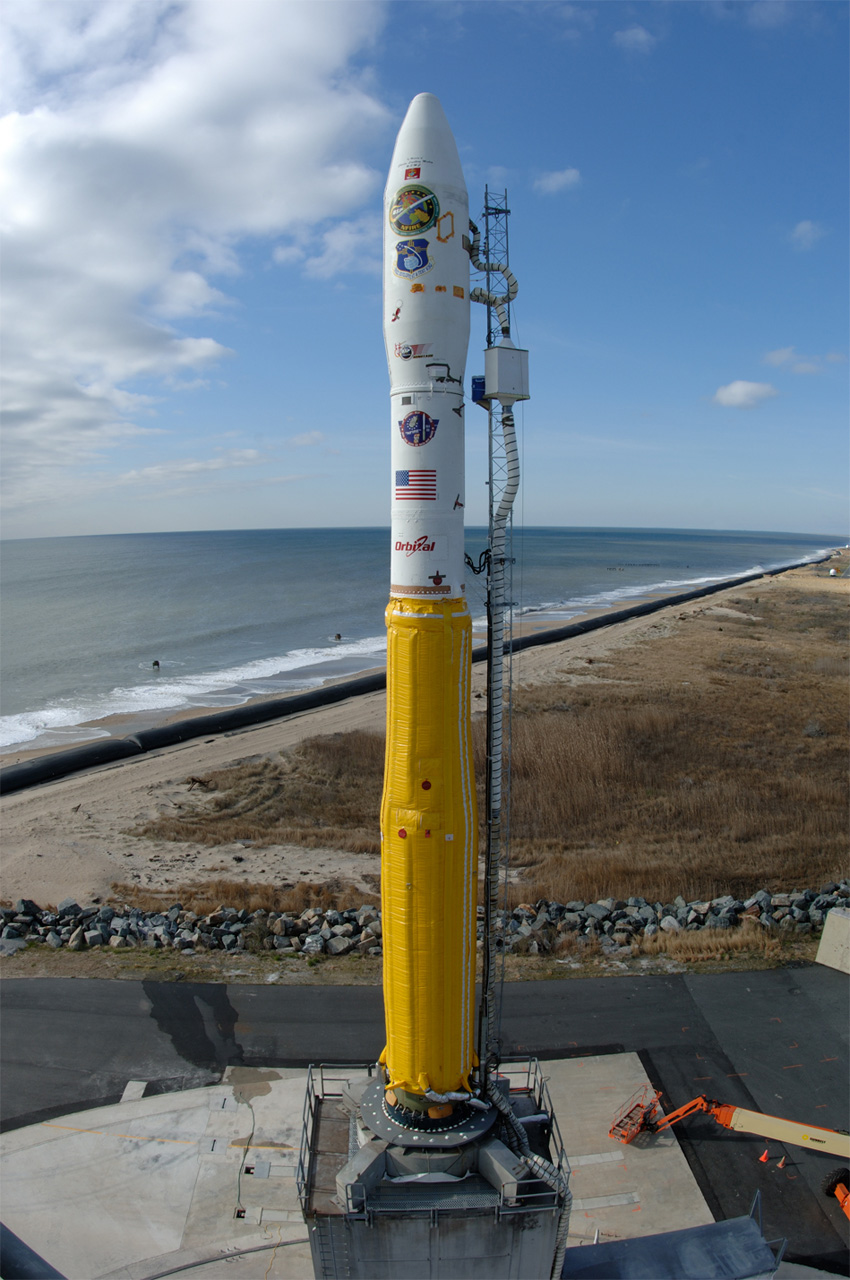
\includegraphics[width=3cm]{content/images/spark/rocket}};
    \node[below left] at (minotaur.north east) {\tiny \textcolor{white}{from Wikipedia/Minotaur-I}};
    \node[xshift=1.8cm,yshift=-3cm,below right] (cubesat) {
      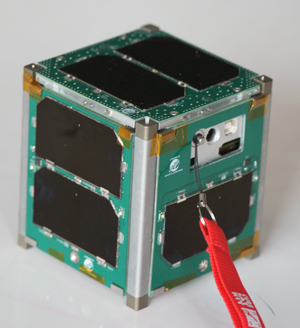
\includegraphics[width=3cm]{content/images/spark/cubesat}};
    \node[above left] at (cubesat.south east) {\tiny \textcolor{white}{from Vermont Tech}};
\end{tikzpicture}
    \end{column}
  \end{columns}
\end{frame}
\addtocounter{clock}{2}

\subsection*{Philosophy}
\begin{frame}[fragile]{The SPARK~2014 Language}
  \framesubtitle{Successor to SPARK~2005. Verifiable subset of Ada language.}
  \begin{itemize}
  \item conceived with verification in mind
  \item imperative language with good tool and platform support
    \begin{itemize}
    \item object-oriented, high re-use
    \end{itemize}
  \item designed for embedded and real-time systems
    \begin{itemize}
    \item run-time checks, strongly typed, inherent support for parallelism
    \end{itemize}

  \item \textbf{principal of minimal surprise}: explicit, easily readable for humans, structural analogies, not case sensitive:
\begin{lstlisting}
Vmax : constant Speed := 12_512.0 * Meter/Second;
\end{lstlisting}

  \item \textbf{difference to C(++):} Getting it to compile is harder, but much less bugs after (longer development time vs. more maintenance)

  \item rated by NIST as approach with ``dramatic future impact'' (reducing
    vulnerabilities by two orders of magnitude)
  \end{itemize}
\end{frame}
\addtocounter{clock}{2}


% \begin{frame}[fragile]\frametitle{Why projects decide for Ada/SPARK}
%   User Reports:
%   \begin{itemize}
%   \item once it compiles, it works $\Rightarrow$ less development time in total (more coding, much less debugging time)
%   \item harder to mix different data types (units, casts, etc)
%   \item programmers have to think harder, which yields better code
%   \end{itemize}
%   Moreover
%   \begin{itemize}
%   \item amenable to static analysis $\Rightarrow$ reduce testing effort
%   \item small memory footprint
%   \item Ada compilers usually have to pass a huge test suite
%     (``ACVC'', > 3,800 tests), whereas almost all C compilers
%     (including gcc) are known to have hundreds of bugs
%   \end{itemize}
% \end{frame}
% \addtocounter{clock}{2}

\subsection*{Pedigree}
\begin{frame}
  \frametitle{Pedigree of SPARK~2014}
  \framesubtitle{Famous users of Ada and SPARK}
  \begin{columns}
    \begin{column}[T]{0.55\textwidth}
      \begin{itemize}
      \item Air Traffic Management: AU, CA, FR, DE, NZ, UK, USA, ...
      \item Civil Aviation: Boeing 777 (99.9\%!), A330, Tu-204, ...
      \item Railway: TGV, ETCS, ...
      \item Rockets: Ariane, Delta, ...
      \item Satellites: INMARSAT, ...
      \item Banking: Reuters, ...
      \item Medical: JEOL Nuclear MRI, LifeFlow VAD, ...
      \item Military: Eurofighter combat aircraft, ...
      \item \dots
      \end{itemize}
    \end{column}
    \begin{column}[T]{0.45\textwidth}
      \vspace*{0cm}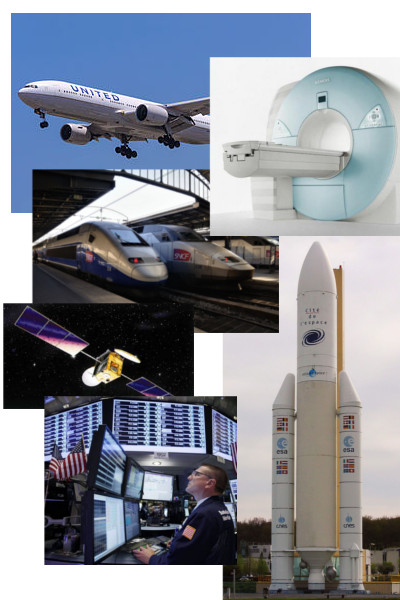
\includegraphics[width=4.5cm]{content/images/spark/users}
    \end{column}
  \end{columns}
\end{frame}
\addtocounter{clock}{2}

\section{Hands-on Part I}
\begin{frame}{Setting up ``Hello World''\hfill(10min)}
Step by step:
  \begin{itemize}
  \item GPS IDE
  \item functions, procedures
  \item packages
  \item variables
  \item Put\_Line (with, use)
  \item if-then
  \end{itemize}
%Final result: \url{http://tinyurl.com/yabb8ktm}
\end{frame}
\addtocounter{clock}{10}

\section{Basic Features}
\subsection{Data Types}

\begin{frame}{Data Types in Ada/SPARK~2014}
\textbf{Strong Type System:} ``I cannot even assign this integer to that other integer...''\\\vspace{1em}

Weakly typed means (C++, C, Java, ...):
\begin{itemize}
\item typedefs are not real types
\item implicit conversions from int to float
\item weak overflow semantics/undefined behavior
\item missing types (fixed-point)
\item two objects of different types can be mixed, although they
  shouldn't: one can add up variables representing \emph{speed} and \emph{time}
\end{itemize}
Ada/SPARK is the opposite.
\end{frame}
\addtocounter{clock}{2}

\begin{frame}
  \frametitle{SPARK~2014: Built-in Types}
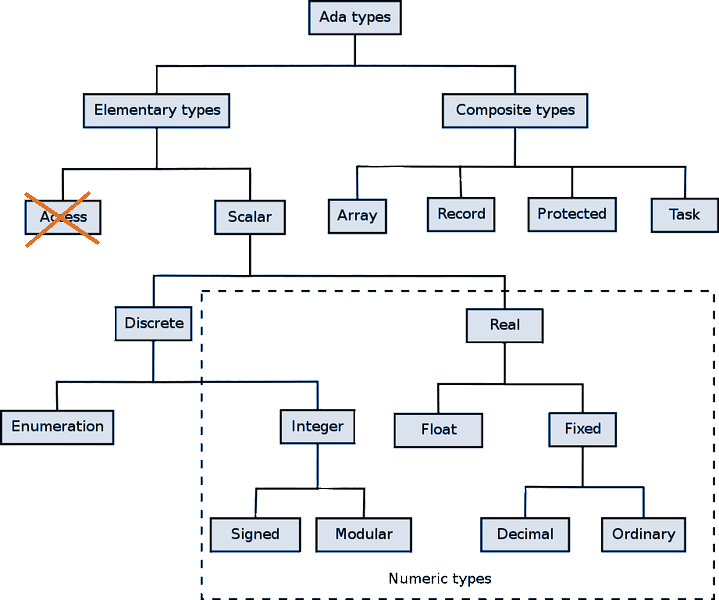
\includegraphics[height=.7\textwidth]{content/images/spark/types}
\footnote{\tiny image (modified) from Ada Wikibooks}
\end{frame}

\begin{frame}[fragile]
  \frametitle{User-Defined Types}
  \begin{itemize}
  \item create a new type based on an existing one. It is \emph{incompatible} to the existing one, but inherits the operations (+,-,*,/,...)
\begin{lstlisting}
type Int_1 is new Integer range 1..10; -- declare type
type Int_2 is new Integer range 1..10; 
var1 : Int_1; -- create object/instance of type
var2 : Int_2;
var1 := var2; -- ERROR: type mismatch
\end{lstlisting}

  \item a \emph{subtype} is compatible to the base type:
\begin{lstlisting}
subtype Integer_1 is Integer range 1..10;
var  : Integer; 
var1 : Integer_1;
var := var1; -- no problem
\end{lstlisting}

  \item way number 3: create new type without base type (nothing inherited)
\begin{lstlisting}
type My_Currency is digits 6;
type My_Enum is (HI, LO, Z);
\end{lstlisting}
%type My_Months is range 1 .. 12; -- confusing
  \end{itemize}
\end{frame}
\addtocounter{clock}{2}

% E.g.:
% \begin{lstlisting}
% package My_Calendar is
%    type Month is Integer range 1..12;
%    type Day is Integer range 1..31;
%    -- ...
% end My_Calendar;
% \end{lstlisting}
% \end{frame}

\subsection{Attributes}

\begin{frame}[fragile]{Attributes}  
  \small
  \vspace{-.5em}
  \begin{itemize}
  \item get/set information about an object
  \item denoted by a single quote, e.g.:
    \begin{itemize}
    \item \texttt{myInteger'First}. Attribute ``First'' returns lowest possible value in this type
    \item \texttt{myInteger'Last}. Returns highest possible value in this type
    \end{itemize}

  \item attribute ``Range'' can be used to iterate over arrays:
    {\scriptsize
\begin{lstlisting}
myArray : array(1..5) of Integer := (2,4,6,8,10);
for i in myArray'Range loop
  -- ...
end loop;
\end{lstlisting}
    }

  \item Attributes ``Succ'' and ``Pred'' can be used to walk through discrete types (e.g., enums, where you cannot do ``+1''):
    {\footnotesize
\begin{lstlisting}
type My_Weekdays is (Monday, Holiday, Friday);
w : My_Weekday := Monday;
w := My_Weekday'Succ (w); -- now we got Holiday
\end{lstlisting}
    }
  \end{itemize}
  {\scriptsize For more see cheat sheet.}

\end{frame}
\addtocounter{clock}{2}

\subsection{Exceptions}

% \begin{frame}[fragile]\frametitle{Exceptions}
%    In case of an unexpected program state
%      \begin{enumerate}
%      \item the control flow of the causing process is interrupted
%      \item the control flow is handed over to an \emph{exception handler}
%      \item if there is no handler, the process terminates
%      \end{enumerate}
%    Typical exceptions:
%    \begin{itemize}
%    \item memory segmentation fault (SIGSEGV): e.g., writing beyond array
%    \item division by zero
%    \item floating-point exception
%    \item ...
%    \end{itemize}  
%    Implemented as software interrupts. \\\vspace{1em}
%    \alert{A well-written program either handles exceptions, or ensures they cannot occur (next lecture)}.
% \end{frame}

\begin{frame}[fragile]\frametitle{Exceptions in SPARK/Ada}
  \begin{itemize}
  \item notify when something is about to go wrong:
    \begin{itemize}
    \item reading beyond an array
    \item assigning a value beyond range of type
    \item ...
    \end{itemize}
  \item many things are checked during run-time
    \begin{itemize}
    \item DIV/0, overflow, array access, range checks, ...
    \item unlike C language (it just continues execution)
    \item (we could disable these checks, but ...)
    \end{itemize}
    
  \item but SPARK~2014 \emph{forbids} the use of exception handlers
  \item forces the developer to handle corner cases explicitly
     \begin{itemize}
      \item unhandled exceptions: program terminated
      \item we must write programs that are free of exceptions
    \end{itemize}
  \end{itemize}
\end{frame}
\addtocounter{clock}{2}

\begin{frame}[fragile]\frametitle{Exceptions in Ada (2)}
The following causes an exception at line 5:
\begin{lstlisting}[escapechar=\`]
 procedure main is
   type mydays is new Integer range 1 .. 31
   d : mydays := 31;
 begin 
   `\tikzmark{s1}`d := d + 1;`\tikzmark{e1}`
   Put_Line("day is:" & mydays'Image(d)); --unreachable
 end main;
\end{lstlisting}
    \begin{tikzpicture}[overlay,remember picture]
      \balloon{s1}{e1}; 
      \node (comment1) [comment] at (\textwidth-.5cm,1.8cm) {beyond type range}; 
      \draw [line] (comment1.west) |- (e1); 
    \end{tikzpicture}

Some exceptions are foreseen by the compiler. Others are not.
\end{frame}
\addtocounter{clock}{1}

\section{Outsmart programmers from IBM and Bell Labs}
\subsection{Binary search}

\begin{frame}
  \frametitle{The binary search algorithm} 
  \framesubtitle{Searching for a number (``key'') in a sorted array, return position}
  
  Example: searching for key=23
  \hspace{3mm}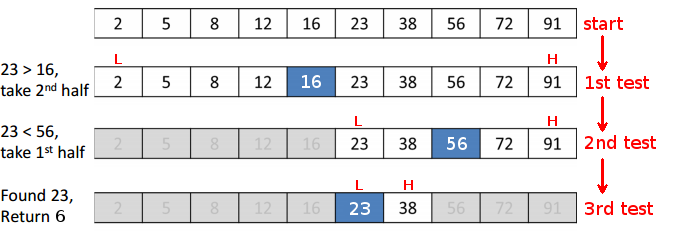
\includegraphics[width=10cm]{content/images/spark/binary-search}\footnotetext{\tiny image (modified) from \url{http://www.geeksforgeeks.org/binary-search/}}
  \begin{enumerate}
  \item \alert L=first element, \alert H=last element
  \item \textcolor{Pantone301}{test element} in the middle of H-L:
    \begin{itemize}
    \item if element = key: found, terminate.
    \item if element < key: repeat search in right half (L=middle+1).
    \item if element > key: repeat search in left half (H=middle-1).
    \end{itemize}
  \end{enumerate}
\end{frame}
\addtocounter{clock}{3}

\section{Hands-on Part II}
\begin{frame}[fragile,fragile]{Binary Search in SPARK \hfill(15min)}
  Start with this skeleton (binary\_search.ads):
\begin{lstlisting}[escapechar=\`]
package Binary_Search is
   type Arr_T is array (`\tikzmark{s1}`Positive`\tikzmark{e1}` range <>) of Integer;

   function Search 
      (Arr : Arr_T; Key : Integer) return `\tikzmark{s2}`Natural;`\tikzmark{e2}`
end Binary_Search;
\end{lstlisting}
main.adb:
\begin{lstlisting}
with Binary_Search; use Binary_Search;
with Ada.Text_IO;   use Ada.Text_IO;
procedure main is 
   arr : constant Arr_T (1..10) := (1,2,4,5,6,7,8,9,10,11);
   idx : Natural;
begin
   -- let's test one case:
   idx := Search (arr, 4);
   Put_Line ("Result is " & Natural'Image(idx));
end main;
\end{lstlisting}
%Write binary\_search.adb yourself, and test some cases.

    \begin{tikzpicture}[overlay,remember picture]
      \balloon{s1}{e1}; 
      \node (comment1) [comment] at (9.5cm,4.0cm) {return zero if\\key not found}; 
      \draw [line] (comment1.west) -| (e1); 
     \balloon{s2}{e2}; 
      \draw [line] (comment1.north) -| (e2); 
    \end{tikzpicture}

%\alert{Copy and paste from: \url{http://tinyurl.com/yash48gs}}
\end{frame}
\addtocounter{clock}{15}

\begin{frame}[fragile,fragile]
  \frametitle{One more Test Case}
Modify your main.adb as follows:
\begin{lstlisting}
Arr (1..Natural'Last) := (Natural'Last => 1, others => 0);
-- ...
idx := Search (arr, 1);
Put_Line ("Result is " & Natural'Image(idx));
\end{lstlisting}

One of many possible mistakes (\texttt{low+high} overflows). Solution?
\begin{lstlisting}
mid := low + (high - low);
\end{lstlisting}
\end{frame}
\addtocounter{clock}{2}

\section{Proof}
\begin{frame}
  \frametitle{Motivation for Proof}
  So far we are only using Ada, but without exception handling.
  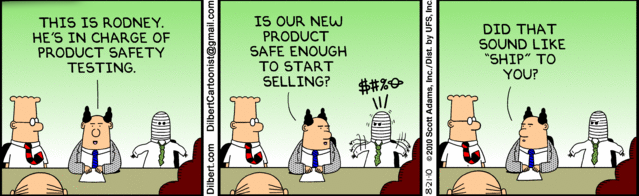
\includegraphics[height=3.1cm]{content/images/spark/testing}\vspace{1em}\\
  Two possible ways forward:
  \begin{enumerate}
  \item use full Ada: handle exceptions, apply testing
  \item use SPARK subset: no exception handling, find \emph{proof}
  \end{enumerate}
  
\end{frame}
\addtocounter{clock}{2}

\begin{frame}
  \frametitle{SPARK~2014: Proof and AoRTE}
  \framesubtitle{Hands-on Intermezzo}
  Launching the verification tool (GNATprove)
  \begin{enumerate}
  \item please add \texttt{with SPARK\_Mode} to your search package (see cheat sheet)
  \item click on menu ``SPARK'' $\rightarrow$ ``Prove All Sources''
  \item select ``Multiprocessing'', ``Report checks proved'' and ``Proof level=2''
  \item click on ``Execute''
  \end{enumerate}
  Finds all defects that could lead to exceptions -- most likely you will have a few red lines now...\\\vspace{1em}
  Fixing all these lines would guarantee \emph{Absence of Run-time Error} (AoRTE)
\end{frame}
\addtocounter{clock}{2}

\begin{frame}
  \frametitle{Verification of SPARK~2014}
  \begin{itemize}
  \item static analysis considers \emph{all possible} inputs and interactions
  \item equivalent to exhaustive testing, but 
    \begin{itemize}
    \item no test harness or fixture necessary
    \item usually much faster than extensive testing
    \item exhaustive testing not possible in real world
    \end{itemize}
  \item some properties are over-approximated, but in a safe way:
    \begin{itemize}
    \item unless verifier finds a proof that bad things are impossible, properties are flagged as failing (red)
    \item e.g.: \texttt{a+b} is classified as overflow, if ranges of \texttt{a} and \texttt{b} are unspecified
    \end{itemize}
  \item sometimes verifier needs a little help (e.g., with loops)
  \end{itemize}
\end{frame}
\addtocounter{clock}{2}

\begin{frame}[fragile]
  \frametitle{Verification of SPARK~2014}
  \framesubtitle{Beyond this tutorial...}
\textit{``Any sufficiently advanced technology\\is indistinguishable from magic.''}\vspace{.4em}\\{\scriptsize Arthur C. Clarke}

      \only<1>{\hspace{4cm}
\includegraphics[height=5cm]{content/images/spark/magic}}
      \only<2>{\hspace{4cm}
\includegraphics[height=5cm]{content/images/spark/magic2}}
\end{frame}
\addtocounter{clock}{1}


\subsection{Contracts}
\begin{frame}\frametitle{Another Type of Error}
  Program works perfectly, for all possible inputs
  \begin{itemize}
  \item no crash, no silent overflows, ...
  \item already better than C++, Java, Rust et al.
  \item<1-1> but \dots
  \item<2-> \vspace{-1.36em}but it could still do the wrong thing
    \begin{itemize}
    \item Not searching at all
    \item search only half of the array
    \item ...
    \end{itemize}
  \item<2-> we need the option to specify intended behavior
  \item<2-> and then also prove it!
  \end{itemize}
\end{frame}
\addtocounter{clock}{2}

\begin{frame}
  \frametitle{Contracts}
  \begin{center}
    
\includegraphics[height=4cm]{content/images/spark/contracts}
  \end{center}

    \begin{itemize}
    \item formal agreement between the implementer and the user of a
      program unit (package or subprogram)
    \item assigns responsibilities
    \item a way to organize and document your code
    \item not a new idea (Floyd, Hoare, Dijkstra, Meyer)
    \end{itemize}
\end{frame}
\addtocounter{clock}{2}

\begin{frame}[fragile]{Pre- and Postconditions}
  \begin{center}
    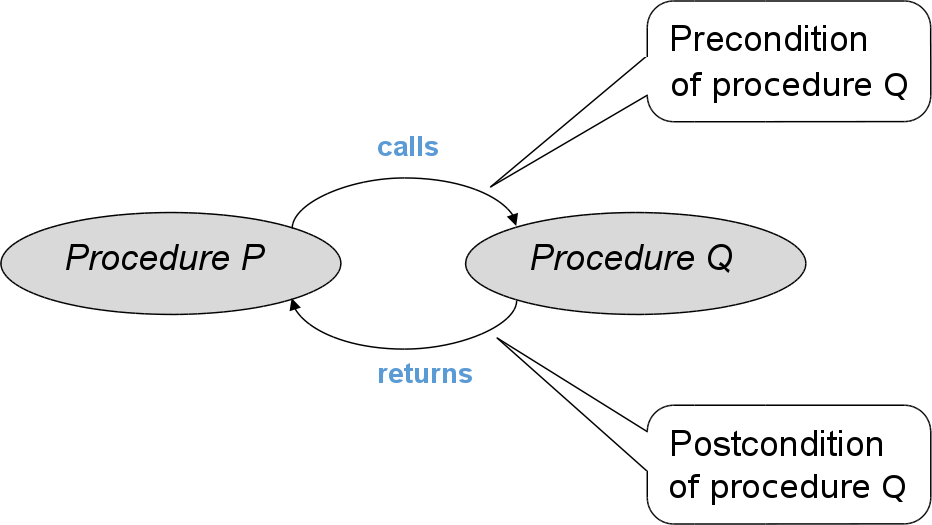
\includegraphics[width=.8\textwidth]{content/images/spark/pre-post}    
  \end{center}
\vspace{-2em}
  \begin{itemize}
  \item are Boolean expressions
  \item \texttt{Pre} is an obligation of the caller
  \item \texttt{Post} is an obligation of the callee
  \item \alert{are verified, just like any other potential exception}
  \end{itemize}
\end{frame}
\addtocounter{clock}{2}


\begin{frame}[fragile]
  \frametitle{Precondition Contracts}
  \begin{itemize}
  \item conditions that must hold true when the subprogram is called
\begin{lstlisting}[escapechar=\`]
-- example:
procedure Increment (X : in out Integer) 
  `\tikzmark{s1}`with Pre => X < Integer'Last;`\tikzmark{e1}`
\end{lstlisting}
    \begin{tikzpicture}[overlay,remember picture]
      \balloon{s1}{e1}; 
      \node (comment1) [comment] at (\textwidth-.7cm,1cm) {precondition}; 
      \draw [line] (comment1.west) |- (e1); 
    \end{tikzpicture}
  \item responsible: caller (must obey these conditions)
  \item verifier tries to \emph{prove} every subprogram call
  \end{itemize}

\begin{lstlisting}[escapechar=\`]
-- our project:
function Search (Arr : Arr_T; Key : Integer) return Natural
  `\tikzmark{s2}`with Pre => Sorted (Arr);`\tikzmark{e2}`

function Sorted (A : Arr_T) return Boolean is 
  (A'Length < 2 or else
    `\tikzmark{s3}`(for all X in A'First .. A'Last - 1 =>
      (for all Y in X + 1 .. A'Last => A (X) <= A (Y))));`\tikzmark{e3}`
\end{lstlisting}%\footnote{\alert{Don't retype that...link to source is provided later!}}
    \begin{tikzpicture}[overlay,remember picture]
      \balloon{s2}{e2}; 
      \node (comment2) [comment] at (\textwidth-0cm,3.7cm) {precondition\\is a Boolean\\function}; 
      \draw [line] (comment2.west) |- (e2); 
     \balloon{s3}{e3}; 
      \node (comment3) [comment] at (\textwidth-0cm,1.6cm) {quantified\\expresssion}; 
      \draw [line] (comment3.south) |- (e3); 
    \end{tikzpicture}
\end{frame}
\addtocounter{clock}{2}

\begin{frame}[fragile,fragile,fragile]
  \frametitle{Postcondition Contracts}
  \begin{itemize}
  \item conditions that must hold true after subprogram finishes
\begin{lstlisting}[escapechar=\`]
-- example:
procedure Increment (X : in out Integer)
  with Pre  => X < Integer'Last,
       `\tikzmark{s2}`Post => X = X'Old + 1;`\tikzmark{e2}`
\end{lstlisting}
    \begin{tikzpicture}[overlay,remember picture]
      \balloon{s2}{e2}; 
      \node (comment2) [comment] at (\textwidth-.5cm,.6cm) {postcondition}; 
      \draw [line] (comment2.west) |- (e2); 
    \end{tikzpicture}
  \item responsible: callee (must provide these conditions)
  \item verifier tries to prove that implementation actually produces these conditions
  \end{itemize}

\begin{lstlisting}
-- our project:
function Search (Arr : Arr_T; Key : Integer) return Natural
  with Pre  => Sorted (Arr),
       Post => (if Search'Result = 0 then True 
                else Arr (Search'Result) = Key);
\end{lstlisting}
\end{frame}
\addtocounter{clock}{2}

\begin{frame}[fragile]{Summary Pre- and Postconditions}
  \begin{center}
    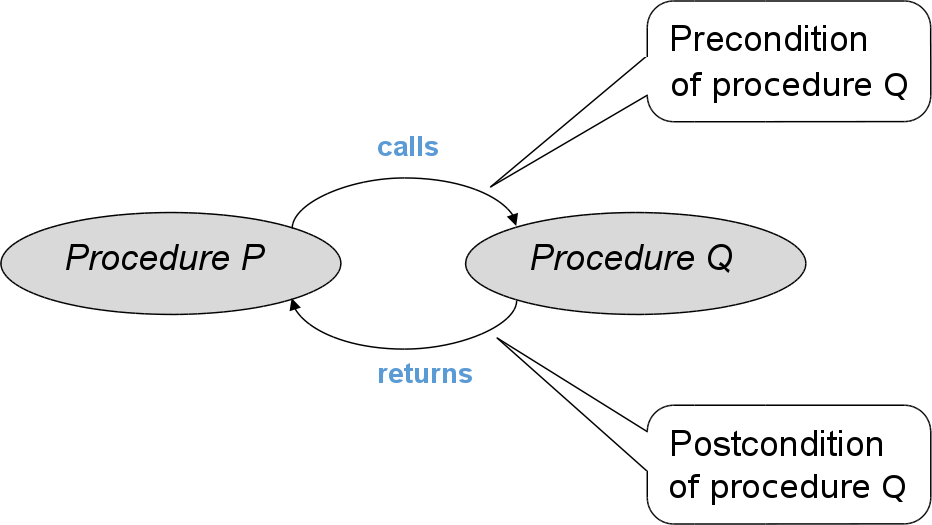
\includegraphics[width=.7\textwidth]{content/images/spark/pre-post}    
  \end{center}
  \vspace{-2em}\begin{itemize}
  \item assign responsibilities
  \item can be composed of
    \begin{itemize}
    \item any visible name in the scope of the subprogram
    \item any parameter of the subprogram
    \end{itemize}
  \item good types simplify contracts (e.g., use \texttt{Natural} instead of \texttt{Integer} when negative numbers are not allowed)
  \end{itemize}
\end{frame}
\addtocounter{clock}{2}

\begin{frame}[fragile]{Modular Verification of SPARK~2014 (1)}
  \begin{center}
    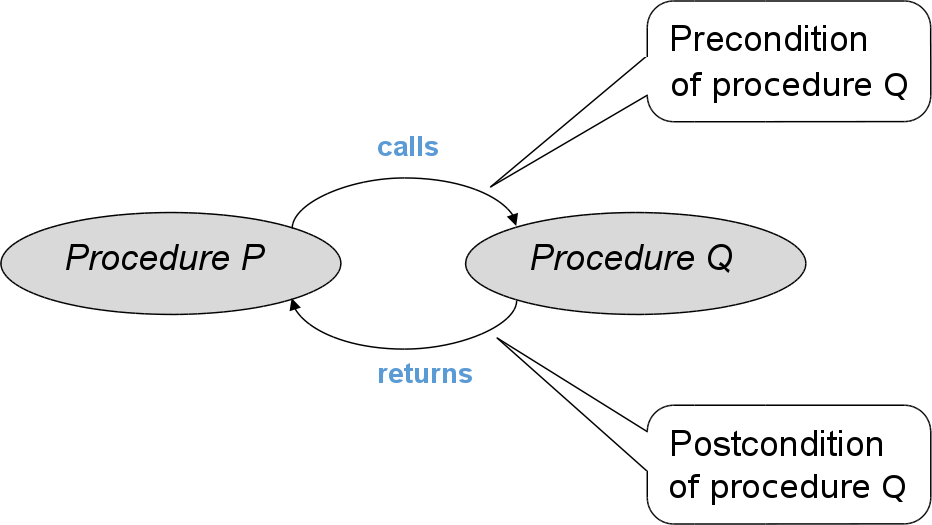
\includegraphics[width=.9\textwidth]{content/images/spark/pre-post}    
  \end{center}
\end{frame}
\begin{frame}[fragile]{Modular Verification of SPARK~2014 (2)} 
  \begin{center}
    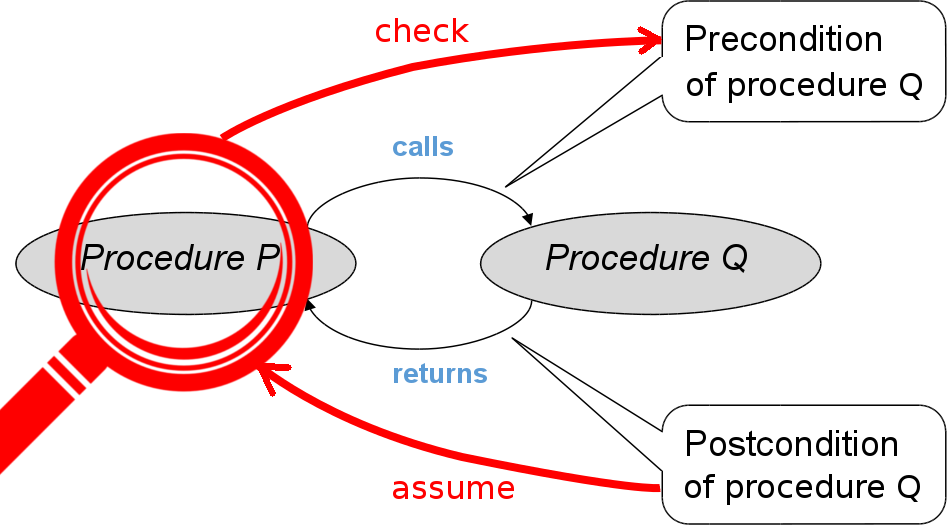
\includegraphics[width=.9\textwidth]{content/images/spark/pre-post-caller}
  \end{center}
  Even if proven free of errors, $P$ may still produce errors when $Q$ violates its postcondition!
\end{frame}
\begin{frame}[fragile]{Modular Verification of SPARK~2014 (3)}
  \begin{center}
    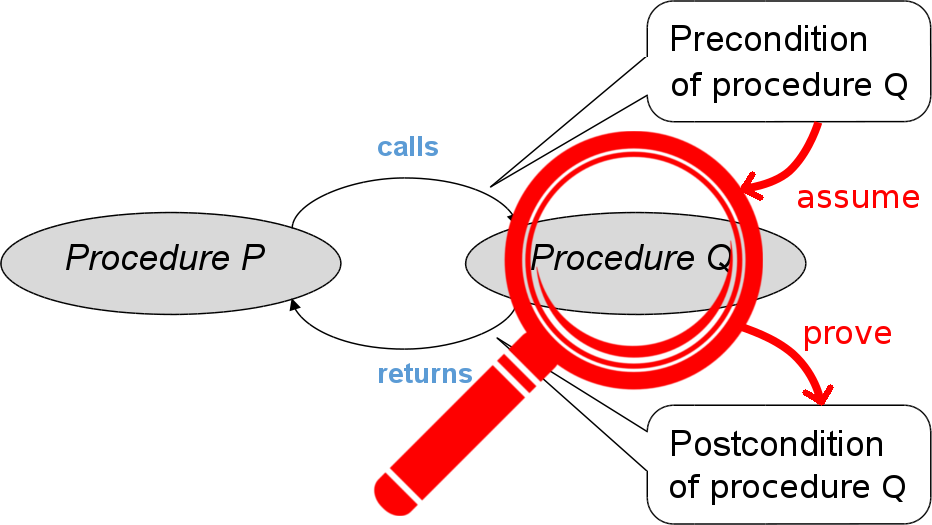
\includegraphics[width=.9\textwidth]{content/images/spark/pre-post-callee}
  \end{center}
Even if proven free of errors, $Q$ may still produce errors when $P$ violates the precondition!
\end{frame}
\addtocounter{clock}{4}

\section{Hands-on Part III}
\begin{frame}[fragile]{Perfecting binary search\hfill (10min)} 
  \begin{itemize}
  \item make use of contracts
  \item time to fix your programs!
  %\item (buggy) implementation so far: \url{http://tinyurl.com/ycz2wk6l}

  \item \alert{array index check might fail: \texttt{Arr(mid) /= Key}}:
  \item loops are notoriously hard to analyze, solver needs hint
  \item add the following into loop to hint solver that \texttt{low, high} should always be in range:
\begin{lstlisting}
pragma Loop_Invariant (low in Arr'Range and 
                       high in Arr'Range);
\end{lstlisting}
  \item solver will \emph{verify} this proposition and then use this fact to get rid of warning
  \end{itemize}
\end{frame}
\addtocounter{clock}{10}

\begin{frame}
  \frametitle{Evaluation of Exercise}
  90\% wrong?\\\vspace{2em}
  Solution: %\url{http://tinyurl.com/y8shbvoo}
  \begin{itemize}
  \item extended postcondition: if result = 0, then key must not be in array
  \item 37 successfully discharged verification conditions in <1s
  \item no exceptions and definitely searching!
  \item all proved without testing
  \end{itemize}
\end{frame}
\addtocounter{clock}{2}

\section{Advanced Topics}

\subsection{Combining Proof and Test}
\begin{frame}
  \frametitle{Combining Proof and Test}  
  \begin{itemize}
  \item sometimes proof may be too expensive
    \begin{itemize}
    \item formal description of all properties may be very hard
    \item Strong postconditions say ``everything'' about the
      subprogram; can't always do that
    \end{itemize}
  \item divide application into pieces and apply either proof or testing to each piece
  \item contracts (and assertions) can be executed (``executable semantics'')
    \begin{itemize}
    \item if program is compiled with assertions on
    \item if they evaluate to False, then exception is raised
    \item contracts can be exercised in a testing environment
    \end{itemize}
  \end{itemize}
\end{frame}
\addtocounter{clock}{3}

\begin{frame}
  \frametitle{Combining Proof and Test (Example)}
  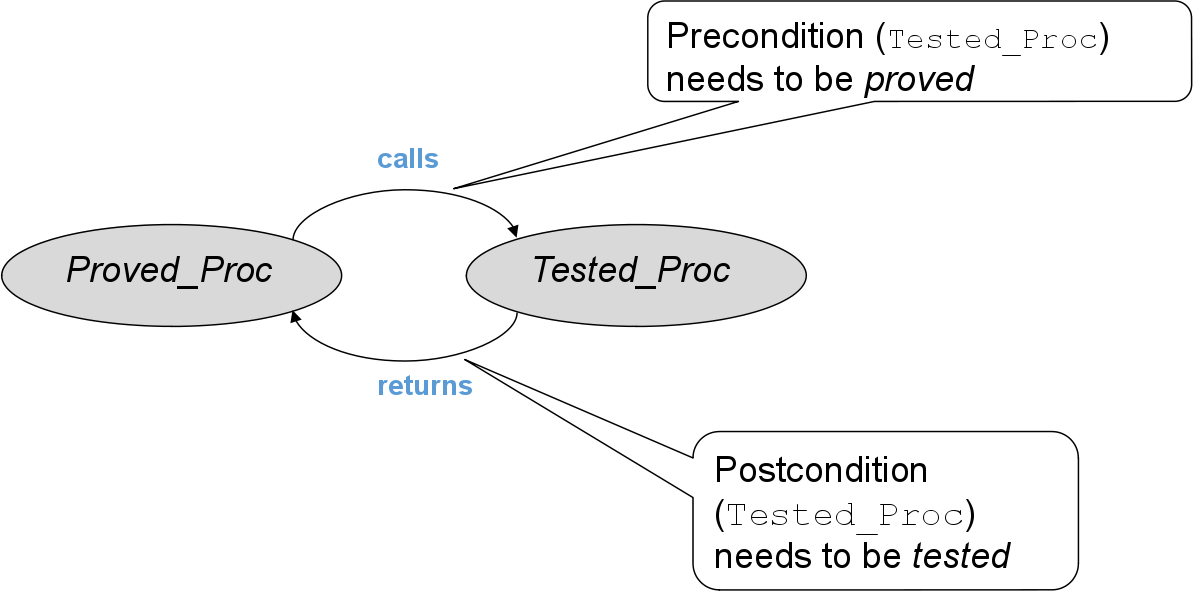
\includegraphics[width=1.\textwidth]{content/images/spark/combining}
\end{frame}
\addtocounter{clock}{1}

\subsection{Real-Time and Safety-Critical}
\begin{frame}{Support for Real-Time and Safety-Critical Software}  
  \framesubtitle{Many things inherited from Ada}
  
  \texttt{with Ada.Real\_Time}
  \begin{itemize}
  \item deterministic scheduling, priority-based interrupt handling, core assignment, preemption, resource sharing protocols
  \end{itemize}
  \texttt{pragma Profile (Ravenscar)}
  \begin{itemize}
  \item constrain tasking features to analyzable subset \& patterns
  \item easier schedulability analysis, memory boundedness, full determinism
  \item memory footprint starting at 2kB $\Rightarrow$ lower certification cost
  \end{itemize}
  Annex ``Safety and Security''/''High-Integrity Systems''
  \begin{itemize}
  \item produce reviewable object code, initialize uninitialized variables to exceptions, option to block specific language features
  \end{itemize}
  Certifiable up to highest assurance levels, e.g., DO-178B Level A for commercial avionics (Level A: failure of software results in catastrophic consequences)
\end{frame}
\addtocounter{clock}{4}
\addtocounter{clock}{3}

\section{Conclusion}
\begin{frame}
  \frametitle{Conclusion}

Catching bugs was never that easy, but it comes with a price. \vspace{1em}\\


\includegraphics[height=3.1cm]{content/images/spark/people}\vspace{2em}\\
Next version of SPARK~2014 under development (pointers!).

\end{frame}

\begin{frame}
  \frametitle{Many Further Topics}  
  \begin{columns}
    \begin{column}[T]{.5\textwidth}
      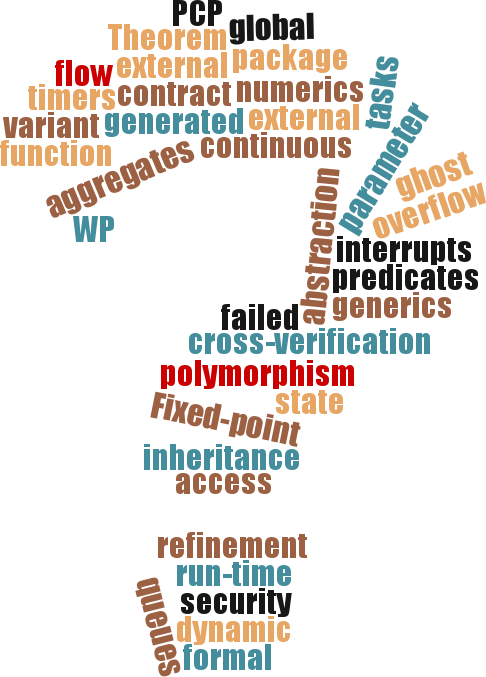
\includegraphics[height=.9\textheight]{content/images/spark/tagcloud}
    \end{column}
    \begin{column}[T]{.5\textwidth}
      
\includegraphics[width=\textwidth]{content/images/spark/sparkbook2}\\
      \begin{center}
        Cambridge University Press, 2015.
      \end{center}
    \end{column}
  \end{columns}
\end{frame}
\addtocounter{clock}{2}

\subsection{References}

\begin{frame}\frametitle{References (1)}
Guides and Tutorials:
{\scriptsize
  \begin{itemize}
  \item \emph{SPARK User Guide}, \url{http://docs.adacore.com/spark2014-docs/html/ug/}
  \item \emph{Ada Wikibook}, \url{http://en.wikibooks.org/wiki/Ada_Programming}
  \item \emph{Ada95 Lovelace tutorial}, David A. Wheeler (who wrote that in his free time), \url{http://www.adahome.com/Tutorials/Lovelace/lovelace.htm}
  \item \emph{Programming Real-Time with Ada 2005}, P. Rogers, \url{http://www.embedded.com/design/prototyping-and-development/4025713/Programming-real-time-with-Ada-2005}, 2006.
  \item \emph{Guide for the use of the Ada Ravenscar Profile in high-integrity systems}, A. Burns et. al., University of York, Technical Report YCS-2003-348, 2003.
  \item \emph{Requiem for a Bug – Verifying Software: Testing and Static Analysis}, Johannes Kanig, Jan 2015, \url{http://www.electronicdesign.com/test-measurement/requiem-bug-verifying-software-testing-and-static-analysis}.
  \end{itemize}
}
\end{frame}

\begin{frame}\frametitle{References (2)}
Background:
{\scriptsize
  \begin{itemize}
  \item \emph{The Boeing 777 Flies on 99.9\% Ada}, \url{http://archive.adaic.com/projects/atwork/boeing.html}
  \item \emph{Ada 95 Eliminates Race Conditions}, J.G.P. Barnes, Parallel and Distributed Real-Time Systems, 1995.
  \item \emph{Ada Glossary}, Bard S. Crawford, \url{http://www.cs.uni.edu/~mccormic/AdaEssentials/glossary.htm}
  \item \emph{GNAT book}, J. Miranda and E. Schonberg, \url{https://www2.adacore.com/gap-static/GNAT_Book/html/aarm/AA-TOC.html}
  \item \emph{Concurrent and Real-Time Programming in Ada}, A. Burns and A. Wellings, Cambridge Univ. Press, 2007.
  \item \emph{Ada 95 Rationale: The Language - The Standard Libraries}, J. Barnes, Springer, 1995.
  \end{itemize}
}
\end{frame}

\begin{frame}\frametitle{References (3)}
Technology behind the scenes:
{\scriptsize
  \begin{itemize}
  \item \emph{RavenSPARK}, R. Chapman, altran praxis, \url{http://www.testandverification.com/files/Multicore_challenge_sept_2010/Rod_Chapman_Altran_Praxis.pdf}, 2010.
  \item \emph{Static Analysis Tools Pass the Quals}, AdaCore, Yannick Moy, 2014.
  \item \emph{The SPARK2014 verifying compiler}, altran, Florian Schanda, 2015.
  \item \emph{Deductive Program Verification with Why3}, J.-C. Filiâtre, DigiCosme Spring School, 2013.
  \end{itemize}
}

\end{frame}


\section{Extra Material (beyond 90')}

\begin{frame}
  \frametitle{The SPARK~2014 Subset}
  \begin{columns}
    \begin{column}[T]{0.5\textwidth}
      Not within SPARK:
      \begin{itemize}
      \item pointers
      \item exception handlers
      \item full Ada tasking (e.g., complex synchronization)
      \item various minor things (e.g., no \texttt{goto})
     \end{itemize}
     Not in Ada:
     \begin{itemize}
     \item certain SPARK-specific aspects (ignored by Ada compiler)
     \end{itemize}
    \end{column}
    \begin{column}[T]{0.5\textwidth}
      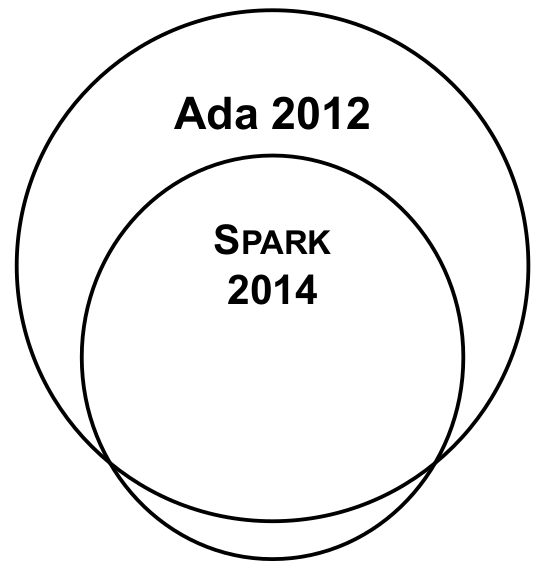
\includegraphics[width=\textwidth]{content/images/spark/subset}
    \end{column}
  \end{columns}
\end{frame}

\subsection{Multi-Threading}

\begin{frame}{Concurrency = Ravenscar Profile}
A ``setting'' that defines a deterministic subset of Ada's tasking capabilities
  \begin{itemize}
  \item restrictions:
    \begin{itemize}
    \item only certain types of synchronization mechanisms (e.g., protected objects)
    \item scheduling policy: FIFO within priorities
    \item static core assignment on multi-core systems
    \item priority ceiling protocol
    \item memory boundedness during link-time
    \end{itemize}
  \item only subset is allowed in SPARK 2014 for tasking
  \end{itemize}
All the details: The \emph{Guide for the use of the Ada Ravenscar Profile in high integrity systems}, A. Burns, B. Dobbing and T. Vardanega, 2003.
\end{frame}

\begin{frame}
  \frametitle{Ravenscar Profile - Task Patterns}
  \framesubtitle{Patterns for Tasks}
Each task must follow one of two implementation patterns:
\begin{enumerate}
\item \textbf{periodic}
  \begin{itemize}
  \item infinite loop with single release point (\texttt{delay until})
  \end{itemize}
\item \textbf{sporadic}
  \begin{itemize}
  \item infinite loop which takes up on an event (interrupt, blocking
    read from queue, ...)
  \end{itemize}
\end{enumerate}
Furthermore:
\begin{itemize}
\item number of tasks must be static
\item tasks must not terminate
\item no hierarchies of tasks
\item \dots
\end{itemize}
\end{frame}

\begin{frame}[fragile]\frametitle{Ravenscar Profile - Tasks, no hierarchy}
  \begin{columns}
    \begin{column}[T]{0.6\textwidth}
      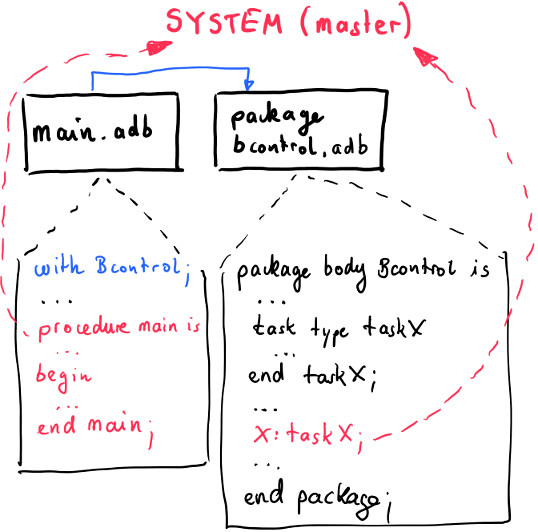
\includegraphics[height=.8\textheight]{content/images/spark/master}
    \end{column}

    \begin{column}[T]{0.4\textwidth}
      \begin{itemize}
      \item tasks are ``all at same level''
      \item scope = package level
      \item master is always the system
      \end{itemize}
    \end{column}
  \end{columns}
\end{frame}


\subsection{Numerical Precision}
\subsection{Floating-Point}
\begin{frame}[fragile]
  \frametitle{Floating-Point Computations (``digits'')}
   \framesubtitle{General Floating point types}
\begin{lstlisting}
type Temperature is digits 18 
   range -173.15 .. 1.41679*10**32;
type Mass is digits 7 
   range 0.0 .. 1.0E35;
\end{lstlisting}
  \begin{itemize}
  \item very weak minimum requirements for float: 
  \item \emph{ideals} (non-numeric values such as \emph{NaN},
    \emph{Inf}) can be excluded
  \item unspecified behavior: Overflow, underflow, zero-divide
  \item at least 6 digits of precision (RM \S3.5.7); towards better portability
    \begin{itemize}
    \item more digits: define own type with \texttt{digits} and optionally \texttt{range}
    \item compiler rejects type if it cannot implement requested precision
    \end{itemize}
  \item semantics of user types are not required to follow IEEE 754
  \end{itemize}
\end{frame}

\begin{frame}[fragile]
  \frametitle{Floating-Point Computations (2)}
  \framesubtitle{\alert{To get proof=reality, we must use IEEE-754 compliant FP computations}}
  \textbf{Built-in Types:} \texttt{Float} and \texttt{Long\_Float}
  \begin{itemize}
  \item floating-point hardware of target may or may not be used 
    \begin{itemize}
    \item GNAT compiler: will use FP hardware
    \item non-GNAT: we can force the compiler to use FPU:
\begin{lstlisting}
Temperature : Interfaces.IEEE_Float_32;
Mass        : Interfaces.IEEE_Float_64;
\end{lstlisting}
    \end{itemize}
  \item hardware may or may not be compliant
    \begin{itemize}
    \item most FPU can/must be configured to be compliant (e.g., disable flush-to-zero)
    \item GNAT: guarantees IEEE-754 semantics on x86 platforms, with flags \texttt{-msse2 -mfpmath=sse} to avoid extended 80bit precision
    \end{itemize}

  \item complete model of Floating-Point arithmetic: RM \S G.2.1.
  \end{itemize}
\end{frame}

\subsection{Interval Arithmetic}
\begin{frame}
  \frametitle{Interval Arithmetic}
  Let $f$ be a numeric operation of $N$ arguments: $f(x_1, x_2, .., x_N)$. Then the corresponding interval operation $F(I_1, I_2, .., I_N)$ is defined as
  \begin{flalign}
    F(I_1, I_2, .., I_N) &= [l,u],\quad\text{where}\\
    l &= \inf\left(f(y_1, y_2, .., y_N)\right)\\
    u &= \sup\left(f(y_1, y_2, .., y_N)\right)\\
    y_i&\in I_i,\; i=1..N 
  \end{flalign}
  $\Rightarrow$ preserve accuracy instead of (usually) precision
  \begin{exampleblock}{Example}
    \vspace{-1em}
    \begin{flalign*}
      z &= y_1 + y_2,\;\text{with } y_i\in[l_i,u_i]\\
        &\Rightarrow z\in [l_1+l_2, u_1+u_2]
    \end{flalign*}
  \end{exampleblock}
\end{frame}

\begin{frame}[fragile]
  \frametitle{Interval Arithmetics (2)}
  Ada library by Dmitry Kazakov, PhD (C.S., software architect) 
  \begin{itemize}
  \item packages define types and overloads operations for tri-state logic, integers and floats.
\begin{lstlisting}
function ``*'' (Left, Right : Interval) return Interval;
function "*" (Left : Interval; Right : Number) return Interval;
function "*" (Left : Number; Right : Interval) return Interval;
\end{lstlisting}
  \item internally using \texttt{Float} and \texttt{Integer} $\Rightarrow$ implementation-defined results
  \item support rounding control (any rounding will produce intervals containing exact result)
  \item source code (GNU) available (e.g., to change to IEEE floats or fixed-point)
  \end{itemize}
  See \url{http://www.dmitry-kazakov.de/ada/intervals.htm} 
\end{frame}

\subsection{Security}
\begin{frame}[fragile]
  \frametitle{Software with Sensitive Data}  
  \begin{itemize}
  \item one problem: when variable with sensitive data is deallocated, memory should be wiped, e.g.:
\begin{lstlisting}
procedure Sensitive_Stuff is 
   x : String := Get_Password();
begin
   -- ...
   x := (others => ' '); -- dead write, optimized out

   -- at this point, memory allocated to x 
   -- shall not hold password anymore
end Sensitive_Stuff;
\end{lstlisting}
  \item use \texttt{volatile} $\Rightarrow$ NO. Slower for \emph{all} reads and writes; not allowed for local variables in SPARK~2014
  \item \texttt{limited type} (not copyable) $\Rightarrow$ pass by ref enforced, solves ownership.
  \item How to wipe memory reliably in the owner?
  \end{itemize}
\end{frame}

\begin{frame}[fragile]
  \frametitle{Software with Sensitive Data (2)}  
  \begin{itemize}
\item \texttt{pragma Inspection\_Point} (from Annex H) $\Rightarrow$
    instructs compiler that object must be \emph{inspectable} (i.e.,
    not optimized out) at given program location
\begin{lstlisting}
x := (others => ' '); -- dead write, optimized out
pragma Inspection_Point (x);
\end{lstlisting}
  \item dead store cannot be optimized out
  \item allows compiler optimization for all other accesses \& provides traceability to registers!
  \item Further: GNATprove detects dead stores and issues warnings $\Rightarrow$ annotate code with suppression = documentation of data sanitization
  \item paper (given below) gives a practical guideline, and discusses many more of this in SPARK~2014
  \end{itemize}
  \footnote{\hspace{-.56cm}\tiny Roderick Chapman, \emph{Sanitizing Sensitive Data : How to Get It Right ( or at Least Less Wrong\dots)}, \\Springer LNCS 10300, 2017.}
\end{frame}